\documentclass[final,dvipdfmx,t]{beamer}

\mode<presentation>
{
	\usetheme{iceberg}
}

\usepackage[orientation=landscape,size=a0,scale=1.4]{beamerposter}
\usepackage[japanese]{babel}
\AtBeginDvi{\special{pdf:tounicode EUC-UCS2}}

\setbeamertemplate{footline}{}

\setbeamerfont{block title}{size=\large,series=\bf}
\setbeamertemplate{navigation symbols}{}
\setbeamertemplate{section in toc}{\inserttocsectionnumber.~\inserttocsection}
\setbeamertemplate{enumerate items}[default]
\setbeamertemplate{itemize items}[default]

\setbeamertemplate{headline}{
	\leavevmode
	\begin{beamercolorbox}[wd=\paperwidth]{headline}
		\begin{columns}[T]
			\begin{column}{.02\paperwidth}
			\end{column}
			\begin{column}{.78\paperwidth}
				\vskip8ex
				\usebeamercolor{title in headline}{\color{iceberg_white}\textbf{\veryHuge{\inserttitle}}\\[1ex]}
				\usebeamercolor{author in headline}{\color{iceberg_blue}\large{\insertauthor}\\[1ex]}
				\usebeamercolor{institute in headline}{\color{iceberg_purple}\large{\insertinstitute}\\[1ex]}
			\end{column}
			\begin{column}{0.06\textwidth}
			\end{column}
			\begin{column}{0.06\textwidth}
			\end{column}
			\begin{column}{.06\paperwidth}
				\vskip1cm
				\vspace{10mm}
				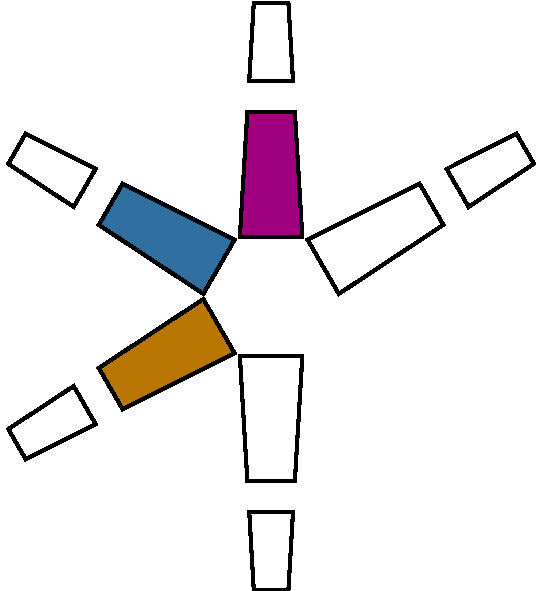
\includegraphics[width=.7\linewidth]{logo-0.pdf}
				\hskip1cm
			\end{column}
			\begin{column}{0.02\textwidth}
			\end{column}
		\end{columns}
		\vskip2ex
	\end{beamercolorbox}
	\vspace{-1em}
}

\title[]{Iceberg for Beamer}
\author[]{enp1s0\inst{1}, tsuki\inst{2} }
\institute[shortinst]{\inst{1} School of Computing, TokyoTech
	\inst{2} Global Scientific Information and Computing Center, TokyoTech}

\begin{document}
\begin{frame}
	\begin{columns}
		\begin{column}{0.485\textwidth}
			\begin{block}{Block 0}
				\begin{itemize}
					\item poi
					\item poi
					\item poi
					\item \alert{alert text}
				\end{itemize}
			\end{block}
			\begin{columns}
				\begin{column}{0.485\textwidth}
					\begin{block}{Block 0-0}
					\end{block}
				\end{column}
				\begin{column}{0.0001\textwidth}
				\end{column}
				\begin{column}{0.485\textwidth}
					\begin{block}{Block 0-1}
					\end{block}
				\end{column}
			\end{columns}
		\end{column}
		\begin{column}{0.485\textwidth}
			\begin{block}{Block 1}
				\begin{enumerate}
					\item poi
					\item poi
					\item poi
					\item poi
				\end{enumerate}
			\end{block}
		\end{column}
	\end{columns}
\end{frame}
\end{document}
